\subsection{Prospectively frozen normal feasibility test}\label{sec:gainpilot}
Before any new attack evaluation, we froze a finite normal-only comparison. The admitted data are the nine exposed Q1/K13 training episodes and nine Q1/M13 development episodes used in the recurrent-model track, each with 1,200 rows and a 100-row warmup. Each role supplies 9,900 eligible targets. L13 calibration, attacks and simulator truth are excluded. Separate observation and command means and standard deviations are fitted only on eligible K13 rows. A common command-only reference uses 16 preceding-command lags, ridge coefficient 0.001 and an unpenalized intercept. This reference is refitted under the common contract; it is not the older ARX commissioning model.

Six constrained adapters cross $\kappa\in\{0.25,0.5,0.75\}$ with $\rho\in\{0.25,0.75\}$. Each has eight hidden units and 200 stored parameters, with $\beta\leq1-\rho$ and $\gamma\leq\kappa$. Trusted context consists of the preceding normalized command and its first difference. The score scale is one for every method. All nine neural fits, including two command-only controls and an unconstrained diagnostic, use seed 17, 40 fixed full-batch Adam epochs, learning rate 0.01 and weight decay $10^{-4}$. Final-epoch weights are retained without development checkpoint selection. Training windows contain 48 burn-in rows and up to 48 scored targets; their zero initialization differs from the full-episode state used for comparative scoring. The windows preserve chronology and do not cross episodes or roles.

The 33-method roster also contains the direct reference, five-lag constrained multivariate residual FIRs, additive command-only-network plus FIR controls, leaky filters, an unconstrained FIR, clipped FIRs and four ordinary residual random-walk Kalman filters. Linear models share protected context and an intercept. The constrained FIR solver projects each output's residual coefficients across all lags onto an $\ell_1$ ball; its exact history gain is the largest such row sum. Command-only nonlinear controls have unrestricted output weights, since their output cancels under the paired comparison. Clipped controls bound only the observation-dependent component. All ten linear fits satisfy the predeclared projected-gradient convergence check.

For normal development, $E_{\rm dev}$ is the largest absolute channel residual and $\tau_{\rm dev}$ is the 99th-percentile maximum-channel score, using sorted zero-based rank 9,800 of 9,900 scores. Substitution into Eq.~\eqref{eq:capradius}, with actual fitted norm bounds, gives an \emph{empirical radius proxy}. It is a selection quantity, not a deployment certificate or independent false-alarm calibration. The candidate and strongest certified comparator are each selected by smallest radius, then RMSE, then a fixed identifier. The registered gate requires at least 5\% lower radius and 2\% lower pooled RMSE against that same comparator, no episode or condition RMSE regression above 5\%, and a lower radius with no worse RMSE than the strongest same-$\kappa$ constrained/additive FIR. Missing convergence, incomplete fits or failed execution checks also block advancement.

\begin{table*}[t]\centering\small\setlength{\tabcolsep}{7pt}
\caption{All 33 normal-development outcomes. $K$ is the actual certified history-gain bound; $C$ bounds the observation-dependent correction for the paired contrast. Radius is the smaller valid gain/cap proxy. A dash means that quantity is unavailable, not zero. All rows use the same 9,900 development targets. ``Late loss drop'' marks more than 1\% training-MSE improvement from epochs 31 to 40; it is not a global convergence test.}\label{tab:gainpilot}
\begin{tabular}{lrrrrc}\toprule
Method & Actual $K$ & Cap $C$ & Radius proxy & RMSE & Late loss drop\\\midrule
Direct reference & 0 & 0 & 3.4098 & 0.11623 & -- \\
Context r=0.25 & 0 & 0 & 3.4178 & 0.11719 & no \\
Context r=0.75 & 0 & 0 & 3.4181 & 0.11715 & no \\
Tanh k=0.25, r=0.25 & 0.25 & 0.25 & 3.6953 & 0.10337 & no \\
Tanh k=0.25, r=0.75 & 0.25 & 0.25 & 3.7866 & 0.10702 & no \\
Tanh k=0.5, r=0.25 & 0.5 & 0.5 & 4.0368 & 0.092446 & no \\
Tanh k=0.5, r=0.75 & 0.5 & 0.5 & 4.1895 & 0.098459 & no \\
Tanh k=0.75, r=0.25 & 0.75 & 0.75 & 4.3733 & 0.083709 & yes \\
Tanh k=0.75, r=0.75 & 0.75 & 0.75 & 4.6067 & 0.091073 & no \\
Unconstrained tanh & 6.3798 & 2.5871 & 6.4328 & 0.040475 & yes \\
FIR k=0.25 & 0.25 & -- & 3.7312 & 0.087017 & -- \\
FIR k=0.5 & 0.5 & -- & 4.4109 & 0.059988 & -- \\
FIR k=0.75 & 0.75 & -- & 6.4616 & 0.037311 & -- \\
Context r=0.25 + FIR k=0.25 & 0.25 & -- & 3.7318 & 0.087007 & -- \\
Context r=0.25 + FIR k=0.5 & 0.5 & -- & 4.4165 & 0.059971 & -- \\
Context r=0.25 + FIR k=0.75 & 0.75 & -- & 6.4615 & 0.03725 & -- \\
Context r=0.75 + FIR k=0.25 & 0.25 & -- & 3.7318 & 0.087007 & -- \\
Context r=0.75 + FIR k=0.5 & 0.5 & -- & 4.4169 & 0.059971 & -- \\
Context r=0.75 + FIR k=0.75 & 0.75 & -- & 6.4616 & 0.037249 & -- \\
Unconstrained FIR & 1.6938 & -- & -- & 0.026939 & -- \\
Clipped FIR C=0.25 & 1.6938 & 0.25 & 3.4167 & 0.082472 & -- \\
Clipped FIR C=0.5 & 1.6938 & 0.5 & 3.4982 & 0.069022 & -- \\
Clipped FIR C=0.75 & 1.6938 & 0.75 & 3.6375 & 0.058067 & -- \\
Leaky k=0.25, r=0.25 & 0.25 & -- & 3.8463 & 0.088432 & -- \\
Leaky k=0.25, r=0.75 & 0.25 & -- & 3.9979 & 0.091762 & -- \\
Leaky k=0.5, r=0.25 & 0.5 & -- & 4.5422 & 0.061615 & -- \\
Leaky k=0.5, r=0.75 & 0.5 & -- & 5.0827 & 0.069441 & -- \\
Leaky k=0.75, r=0.25 & 0.75 & -- & 6.7292 & 0.03791 & -- \\
Leaky k=0.75, r=0.75 & 0.75 & -- & 8.8905 & 0.052101 & -- \\
KF q/r=0.01 & 1 & -- & -- & 0.072175 & -- \\
KF q/r=0.1 & 1 & -- & -- & 0.043984 & -- \\
KF q/r=1.0 & 1 & -- & -- & 0.029287 & -- \\
KF q/r=10.0 & 1 & -- & -- & 0.025881 & -- \\
\bottomrule\end{tabular}

\end{table*}

\subsection{Outcome and interpretation}
The gate fails (Table~\ref{tab:gainpilot}). The selected adapter has $\kappa=\rho=0.25$. Its RMSE is 0.10337 versus 0.11623 for the selected direct-reference comparator, an 11.06\% reduction. Its radius proxy is nevertheless 3.69533 versus 3.40982, an 8.37\% increase rather than the required 5\% reduction. The same-budget FIR has RMSE 0.08702, better than the candidate, although its radius of 3.73124 is slightly larger. Thus both the primary radius condition and the same-budget RMSE condition fail; the episode/condition regression and implementation clauses pass.

The selected adapter's gain-only proxy is 4.26044. Its smaller reported value comes from the ordinary amplitude-cap argument. This matters because saturation is also available to a simple control. The clipped FIR with $C=0.25$ has radius 3.41671 and RMSE 0.08247, both smaller than the selected neural values. A descriptive check of the complete prespecified roster finds that this same clipped FIR dominates all six constrained neural candidates on both quantities. All six candidates obtain their tighter proxy from the amplitude cap, not the gain bound. These observations preserve the original failed criterion. Figure~\ref{fig:gainpilot} shows the radius/error trade-off and all neural training histories.

\begin{figure*}[t]\centering
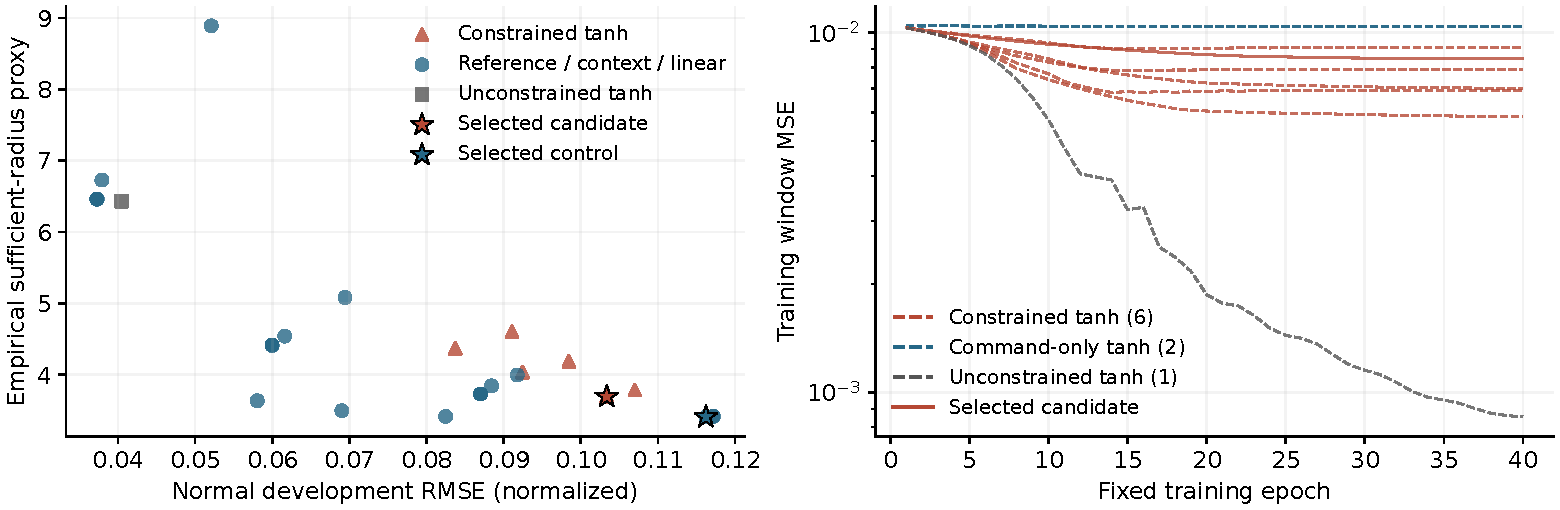
\includegraphics[width=0.94\textwidth]{figures/gain_feasibility.pdf}
\caption{Normal-only feasibility. Left: every method with a finite radius proxy; methods without one remain in Table~\ref{tab:gainpilot}. Stars mark the candidate and comparator chosen by the predeclared rule. Lower values are preferred on both axes. Right: all nine fixed 40-epoch training histories. These are exposed development and training results, without attack outcomes, confidence intervals or an operational guarantee.}\label{fig:gainpilot}
\end{figure*}

The selected adapter does not trigger the predeclared late-improvement flag. One other constrained adapter and the unconstrained neural diagnostic do. Neither flag state proves global optimization, and this finite run does not establish that every possible nonlinear model is inferior. It rejects advancement of this specified candidate under the declared criteria. No threshold calibration, fresh attack campaign, longer training or criterion revision follows the failure.

All 33 methods, nine neural fits and ten linear fits complete in one monitored run: 5.696 s wall, 4.810 CPU seconds, 292.4 MB sampled peak RSS and 23.69 MB output, within 120 s, 90 CPU seconds, 1 GiB and 50 MiB. Sixteen synthetic software tests pass before the 41-identity freeze. Reloaded weights reproduce all neural predictions exactly in PyTorch. A separate NumPy implementation differs by at most $2.39\times10^{-7}$ and independently reconstructs the norms, metrics, linear stationarity checks and failed decision without importing the model/evaluation helpers. Source/input identities, every fitted model, epoch history, normalized development record and prediction are retained. Runtime was conservatively admitted from a synthetic tensor fixture before research-data fitting; the fixture was not robot evidence. These AI-assisted checks support the execution record, not independent human replication or physical generalization.
